%%%%%%%%%%%%%%%%%%%%%%%%%%%%%%%%%%%%%%%%%
% Dreuw & Deselaer's Poster
% LaTeX Template
% Version 1.0 (11/04/13)
%
% Created by:
% Philippe Dreuw and Thomas Deselaers
% http://www-i6.informatik.rwth-aachen.de/~dreuw/latexbeamerposter.php
%
% This template has been downloaded from:
% http://www.LaTeXTemplates.com
%
% License:
% CC BY-NC-SA 3.0 (http://creativecommons.org/licenses/by-nc-sa/3.0/)
%
%%%%%%%%%%%%%%%%%%%%%%%%%%%%%%%%%%%%%%%%%

%----------------------------------------------------------------------------------------
%	PACKAGES AND OTHER DOCUMENT CONFIGURATIONS
%----------------------------------------------------------------------------------------

\documentclass[final,hyperref={pdfpagelabels=false}]{beamer}
\usepackage[utf8]{inputenc}
\usepackage{multirow}
\usepackage[orientation=portrait,size=a1,scale=1.8]{beamerposter} % Use the beamerposter package for laying out the poster with a portrait orientation and an a0 paper size
\usepackage{xcolor}
\usetheme{I6pd2} % Use the I6pd2 theme supplied with this template
%\usepackage{extsizes}
\usepackage[french]{babel} % English language/hyphenation

\usepackage{amsmath,amsthm,amssymb,latexsym} % For including math equations, theorems, symbols, etc

%\usepackage{times}\usefonttheme{professionalfonts}  % Uncomment to use Times as the main font
%\usefonttheme[onlymath]{serif} % Uncomment to use a Serif font within math environments

\boldmath % Use bold for everything within the math environment

\usepackage{booktabs} % Top and bottom rules for tables

\graphicspath{{figures/}} % Location of the graphics files

\usecaptiontemplate{\small\structure{\insertcaptionname~\insertcaptionnumber: }\insertcaption} % A fix for figure numbering

%----------------------------------------------------------------------------------------
%	TITLE SECTION 
%----------------------------------------------------------------------------------------

\title{\huge Integrated mini-cloud of RaspberryPIs for distributed systems training} % Poster title

\author{Monroe Samuel, Voet Rémy \\
Director: Étienne Rivière} % Author(s)


\institute{UCLouvain} % Institution(s)

%----------------------------------------------------------------------------------------
%	FOOTER TEXT
%----------------------------------------------------------------------------------------

\newcommand{\leftfoot}{Open source project} % Left footer text

\newcommand{\rightfoot}{https://github.com/splay-project-v2} % Right footer text

%----------------------------------------------------------------------------------------

\begin{document}

\addtobeamertemplate{block end}{}{\vspace*{2ex}} % White space under blocks

\begin{frame}[t] % The whole poster is enclosed in one beamer frame

\begin{columns}[t] % The whole poster consists of two major columns, each of which can be subdivided further with another \begin{columns} block - the [t] argument aligns each column's content to the top

\begin{column}{.02\textwidth}\end{column} % Empty spacer column

\begin{column}{.465\textwidth} % The first column
            
\begin{block}{Objectives}
Testing \textbf{distributed algorithms} in real condition, get feedback, with an easy-to-use integrated solution.
\begin{itemize}
    \item Easy usage through a \textbf{web-app}.
    \item User implements distributed algorithm using a concise \textbf{Lua}-based language.
    \item Distributed algorithm \textbf{performance} and \textbf{robustness} test.
    \item Guided \textbf{assignment} by professor for student.
\end{itemize}

\end{block}

\begin{block}{Features}

\begin{itemize}
    \item \textbf{Fault injection} to test robustness of a distributed algorithm
    \item \textbf{Network} topology \textbf{editor}
    \item \textbf{Performance measurement} of the algorithm for each node
    \item \textbf{Lua} Script \textbf{editor}
    \item \textbf{Modern} web-app
\end{itemize}

\end{block}

\begin{block}{Cluster of RaspberryPIs}
\noindent
\begin{figure}
    \centering
    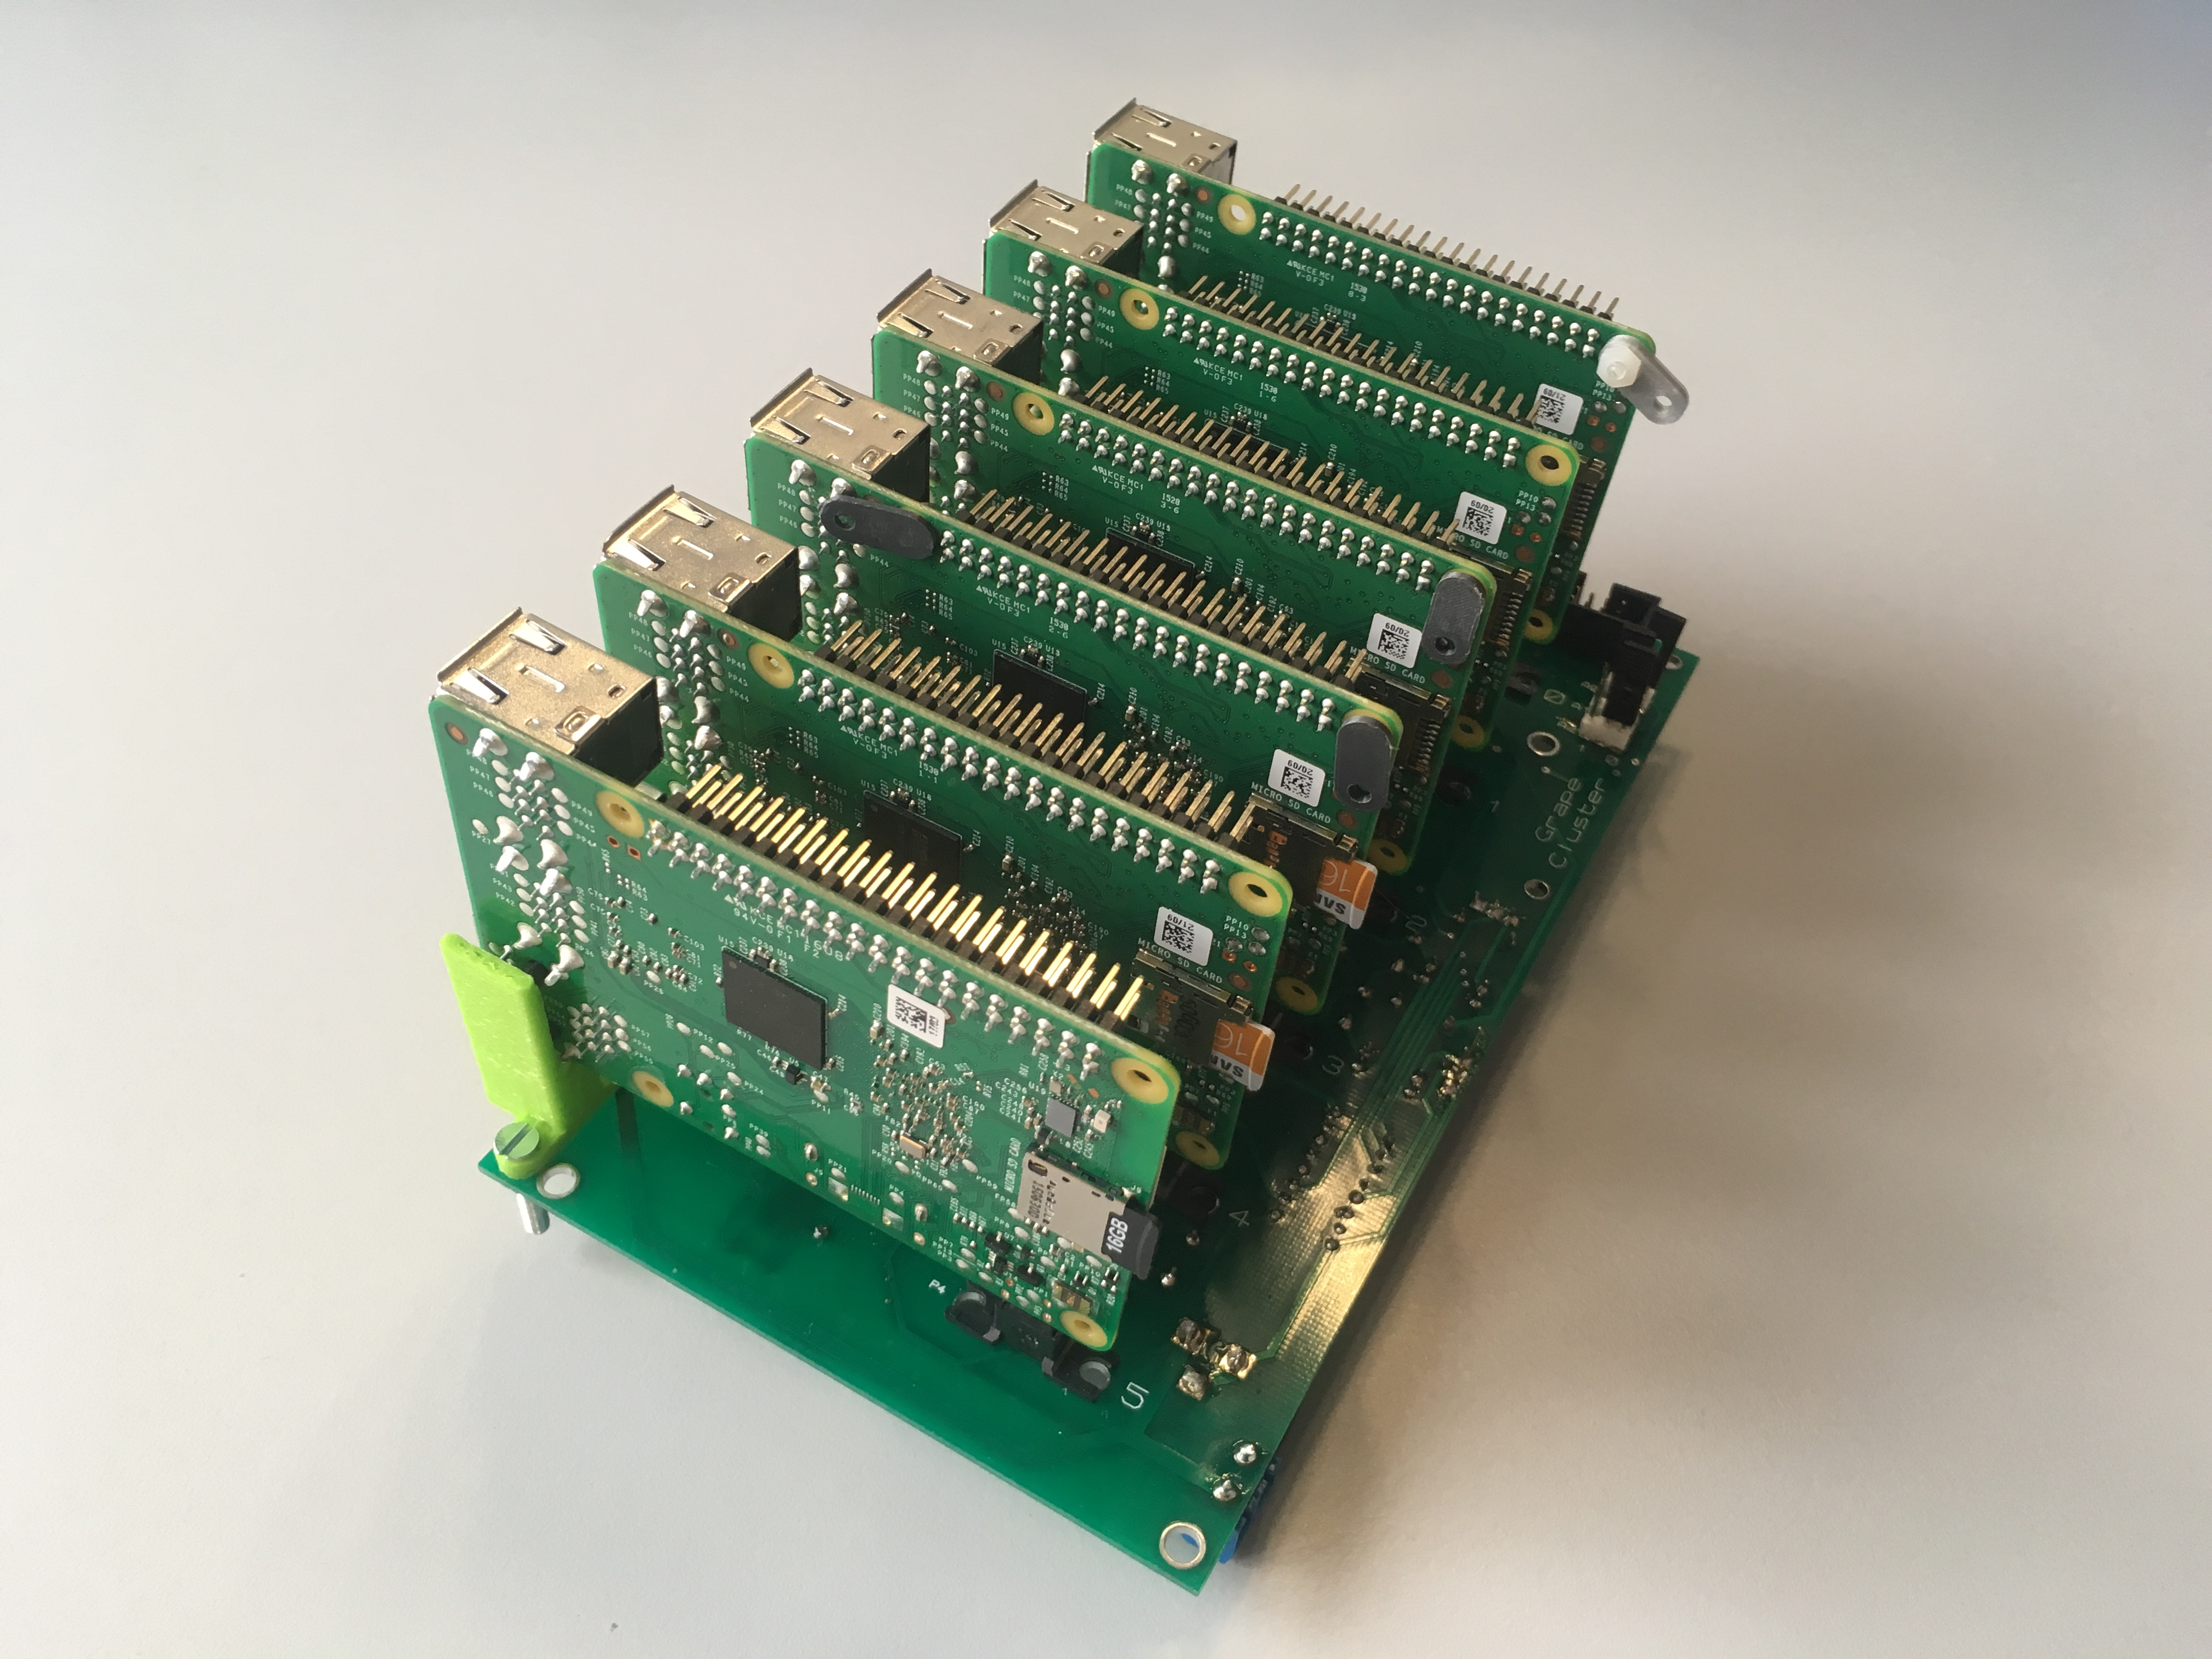
\includegraphics[scale=0.13]{rasp_stack.jpg}
\end{figure}

\end{block}

% \begin{block}{Project quality}
% \begin{itemize}
%     \item One-Click install
%     \item Automatic features testing 
%     \item Scalable model
%     \item Clear and complete documentation
% \end{itemize}
% \end{block}
\begin{block}{Usage scenario}
You want to compare two consensus algorithm (paxos vs raft) : 
\begin{itemize}
    \item Download the \textbf{web-app} from master PI
    \item Create your \textbf{Lua scripts} with the integrated editor
    \item Create your own \textbf{network topology} (or use a default one)
    \item Put your \textbf{fault injection} into the code (meta-parameters)
    \item Test your algorithm in \textbf{semi-real condition}
    \item Get \textbf{performance} and  \textbf{custom logs} of each node
    \item Retry with different settings
\end{itemize}
\end{block}


%------------------------------------------------

\end{column} % End of the first column
\begin{column}{.03\textwidth}\end{column} % Empty spacer column
 
\begin{column}{.465\textwidth} % The second column


\begin{block}{Model}

\noindent
\begin{figure}
    \centering
    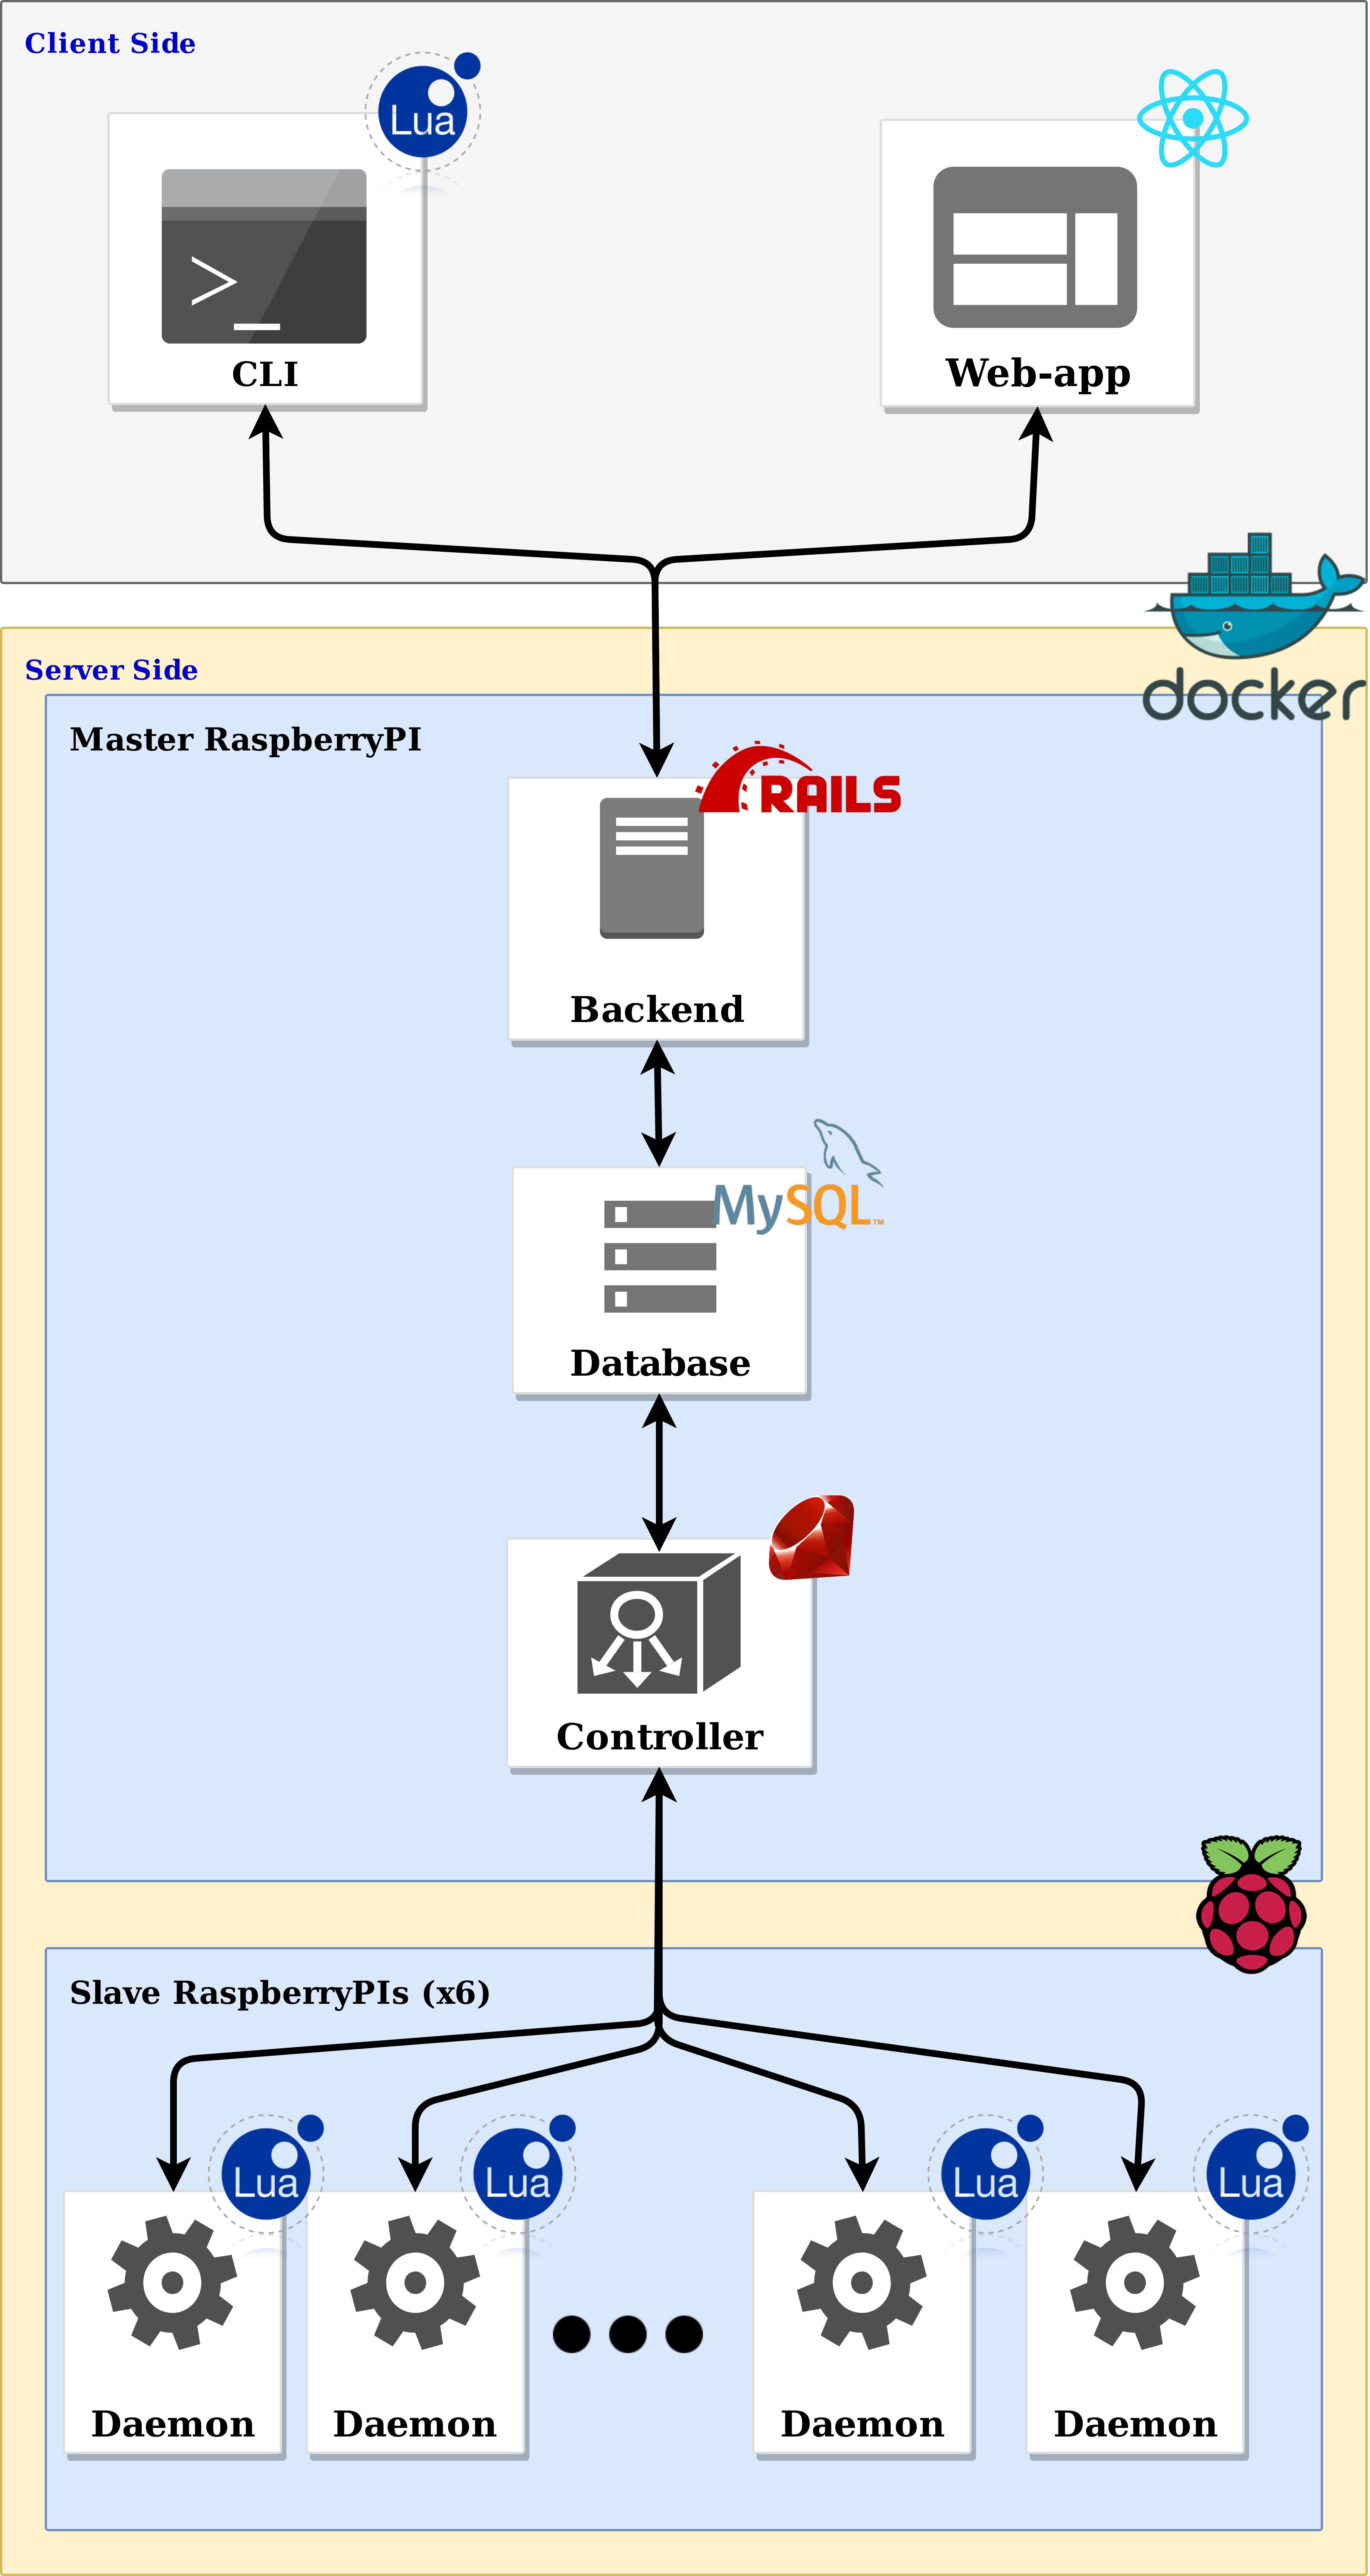
\includegraphics[scale=0.203]{SplayNewIcon.png}
\end{figure}

\end{block}


\begin{block}{Planning}

\begin{itemize}
    \item \textbf{20/01} : Finish/Clean the upgrade from the old project (version of Ruby, Rails, Lua).
    \item \textbf{01/02} : Automatic testing of the old project (each part)
    \item \textbf{15/02} : Modern Web-app and Lua script editor
    \item \textbf{22/02} : Fault injection and performance measurements
    \item \textbf{08/03} : Network topology editor
\end{itemize}

\end{block}

\end{column} % End of the second column

\begin{column}{.015\textwidth}\end{column} % Empty spacer column

\end{columns} % End of all the columns in the poster

%----------------------------------------------------------------------------------------
%----------------------------------------------------------------------------------------
%	CONCLUSION
%----------------------------------------------------------------------------------------

%----------------------------------------------------------------------------------------
\begin{center}
\color {white}
\textbf{samuel.monroe@student.uclouvain.be - remy.voet@student.uclouvain.be}
\bigskip
\end{center}
\end{frame} % End of the enclosing frame

\end{document}